\lab{Application}{Single Pixel Camera}{Single Pixel Camera}
\label{lab:SPC}

\objective{You will build a single pixel camera that to take pictures of 2d and 3d tessellations.}

\section*{Single Pixel Camera}
When you look at a picture on a computer screen it is divided into areas called pixels. Each pixel is a square that has a Red-Green-Blue (RGB) color value. When a  modern digital camera takes a picture it divides the picture in to pixels and stores the amount red, green, and blue light that comes in at each square.

A single pixel camera treats the whole image as one pixel and thus only stores one RGB value that is the average color value of the whole image.  

\section*{2D Images}
In this lab we are going to represent the pictures as tessellated image. A tessellated image is a tiling with geometric shapes with no overlaps or gaps. 

In this lab we assume that $\mathcal{S}$ has a given tessellation $\mathcal{T} = \{F_i\}$, where $F_i$ represents a particular face of our tessellation. Without loss of generality, we will assume that each $F_i$ is a triangle. We will represent the vertices of $F_i$ by $F^j_i$, where $F^j_i$ will be a column vector of length two representing the coordinates of $F_i$.

Recall from multivariable calculus that the area of a triangle is half the magnitude of the cross product. For $F_i$ this is given by
\begin{align}
v_1 &= F_i^1 - F_i^0 \\
v_2 &= F_i^2 - F_i^0 \\
A_i &= \frac{1}{2}\big|v_1[0] v_2[1] - v_1[1] v_2[0]\big|
\end{align}


We represent our signal, in this case our RBG color values, as a vector $s$, where the length of $s$ is the number of faces of our tessellation $\mathcal{T}$. We assume, naturally, that the value of our signal  on the face $F_i$ is exactly the value $s[i]$. We can then, using the areas previously calculated, express the single-pixel measurement of the signal of the camera as an inner product:
\begin{equation}
A \cdot s = b
\end{equation}
In addition, we assume that the total area of the image is equal to the sum of our tessellation. So  
\begin{equation}
\hat{b} = \frac{b}{\sum_i A_i}
\end{equation}

Then $\hat{b}$ will be the RGB values of the singe pixel.

\begin{problem}
Write a function that takes in $S$, a 3-d array of the vertices of 2d tessellation faces, and $s$ , the RBG values of the each tessellation. Output the RGB value given by the single pixel camera. Below is code to visualize the tessellation and $\hat{b}$.  Also included below is test code.
\end{problem}

\begin{lstlisting}
import matplotlib.pyplot as plt
from matplotlib.collections import PolyCollection
# This function plots a 2D tesselation, S, with the colors s 
def visualize2d(S,s):
    fig, ax = plt.subplots()
    coll = PolyCollection(S, facecolors=s)
    ax.add_collection(coll)
    ax.autoscale_view()
    plt.show()
\end{lstlisting}
\begin{lstlisting}
#Let b be a 1d array of 3 values representing the RGB values. This plots the color
plt.imshow(np.array([[b]]))
plt.show()
\end{lstlisting}
\begin{lstlisting}
#if your solution to problem 1 was called SPC2, your code should run similarly
test=np.array([[[.5,0],[0,1],[0,0]],[[.5,0],[0,-1],[0,0]],
               [[-1,0],[0,1],[0,0]],[[-1,0],[0,-1],[0,0]]])
C=np.array([[0,0,1],[1,0,0],[0,1,0],[1,0,1]])
SPC2(test,C)
>>> array([ 0.5,  0.3333, 0.5])
\end{lstlisting}

\section*{Projective Transforms}
Now say that we have a tessellated 3d object and we would like to take a single pixel picture of it.

We begin by selecting a random camera location $c$. The location is selected randomly on a sphere centered at the origin, with norm large enough that the entire surface lies inside the sphere. The camera is assumed to point directly at the origin.

In order to keep the distance of the camera from the origin constant, this is best done by inputting the spherical coordinates and then changing to rectangular. Recall the that the formula to change polar coordinates to rectangular is 
\[
S(\theta,\phi,r)=(r*\sin(\phi)*\cos(\theta),r*\sin(\phi)*\sin(\theta),r*\cos(\phi))
\theta \in [0,2\pi),\phi \in [0,\pi), r \in [0,\infty)
\]
\begin{problem}
Write a function that changes spherical coordinates to rectangular.
\end{problem}

We then utilize the projective transform to calculate how the camera ``sees'' the faces of the surface. Here we state the appropriate equations:

\begin{align}
t &= \text{acos}(\frac{-c_2}{\|c\|}) \\
w^* &= \begin{bmatrix}
	\frac{c_1}{\|c\|} \\
	\frac{-c_0}{\|c\|} \\
	0
\end{bmatrix} \\
w &= \frac{w^*}{\|w^*\|} \\
\hat{w} &= \begin{bmatrix}
0 & 0 & w_1 \\
0 & 0 & -w_0 \\
-w_1 & w_0 & 0
\end{bmatrix} \\
R &= e^{\hat{w}t} = I + sin(t) \hat{w} + (1-cos(t)) \hat{w}^2 \\
P &= \begin{bmatrix}
R^T & -R^T c \\
0 & 1
\end{bmatrix}
\end{align}

We can then use the matrix $P$ to transform any point $x$ in homogenous world, in this case homogenous coordinates are created by simply appending 1 to the bottom of a given column vector, coordinates to homogenous camera coordinates $y$ by the equation:
\begin*{equation}
Px = y
\end*{equation}

\begin{problem}
Write a function that takes in a camera location and outputs the transformation matrix.
\end{problem}

We can then find the projective transform (i.e. how the camera ``sees'' a point) by the equation:
\begin{equation}
P_c(y) = \begin{bmatrix}
\frac{y[0]}{f \cdot y[2]} \\
\frac{y[1]}{f \cdot y[2]}
\end{bmatrix}
\end{equation}

Here $f$ represents the distance from the camera to the image plane, which is essentially an arbitrary constant. I recommend using $f=.5$.

\begin{problem}
Write a function that takes in a transformation matrix, a list of points in world coordinates, and a constant $f$ and outputs the projective transform of the points.
\end{problem}

\begin{figure}
\begin{subfigure}{.49\textwidth}
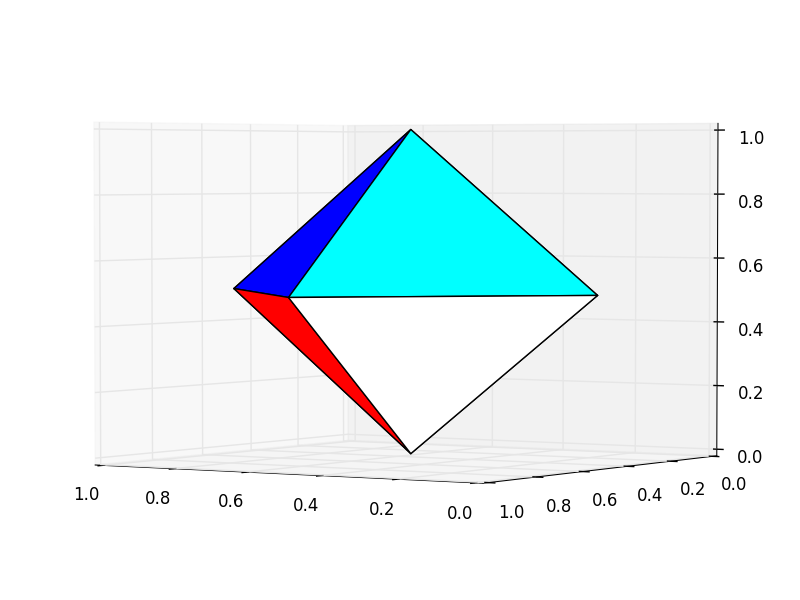
\includegraphics[width=\textwidth]{3dbefore.png}
\end{subfigure}
\begin{subfigure}{.49\textwidth}
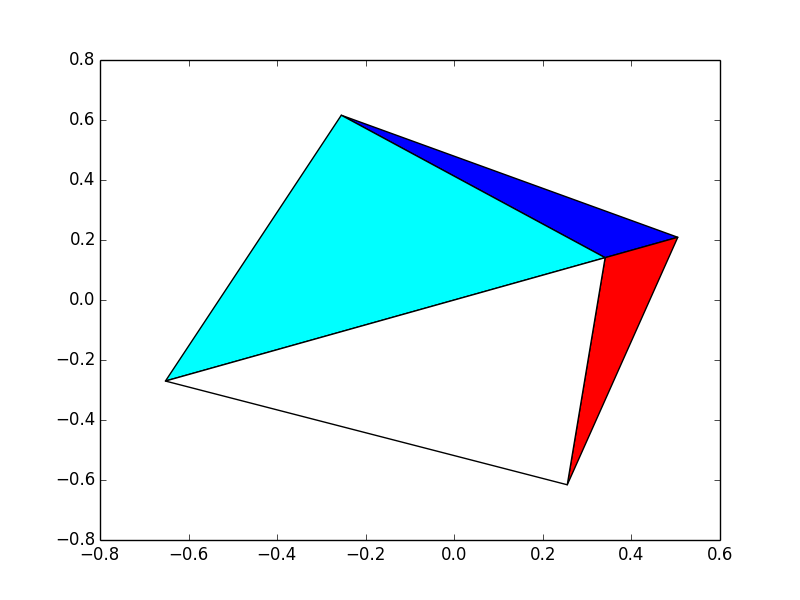
\includegraphics[width=\textwidth]{projection.png}
\end{subfigure}
\caption{3d tesselation and its projection}
\label{fig:proj}
\end{figure}

Now we essentially we have 2d points and we can calculate the areas as we did in the 2d case. Now we have the areas of each face of our tessellation with respect to our camera view. One thing that we need to worry about is the visibility of the face $F_j$. This constant, for convex surfaces, will either be zero or one. In this case the constant, if the center of the face denoted $Fc_j$ and $r$ is the radius of the tessellation. Then
\[
e_j=||c-Fc_j||_2<\sqrt{||c||_2^2+r^2}-\epsilon
\] 
Where $\epsilon$ is small (I recommend .2 if the camera distance is 3).
Then $e_j$ is a constant representing the  the visibility of of the face $F_j$.

\begin{problem}
Write a function that takes in an array of vertices of a tessellation, a camera position, the radius of the tessellation, and an $\epsilon$ value and outputs an array of visibility constants.
\end{problem}
Then:

\begin{equation}
M(j) = A_j \cdot e_j
\end{equation}
Then
\begin{equation}
M \cdot s = b
\end{equation}
\begin{equation}
\frac{b}{\sum_j M_j} = \hat{b}
\end{equation}
And $\hat{b}$ is the RGB value of a picture taken by the single pixel camera at location $c$.

\begin{problem}
Using the previous problems, write a function that takes in an array of vertices of a tessellation, color values for the faces of the tessellation and a camera position in spherical coordinates and outputs single pixel RGB value. Below is plotting script for 3d tessellations. Included is data from a satellite that makes a tessellation of the earth, Use it to test your function.
\end{problem}

\begin{lstlisting}
import matplotlib.pyplot as plt
from mpl_toolkits.mplot3d import Axes3D
from mpl_toolkits.mplot3d.art3d import Poly3DCollection
import matplotlib.colors as colors
# This function plots a 2D tesselation, F, with the colors C. 
def visualize3d(F,C):
    fig = plt.figure()
    ax = Axes3D(fig)
    l=len(F)
    for n in xrange(l):
        verts = [zip(F[n,0]*.5+.5,F[n,1]*.5+.5,F[n,2]*.5+.5)]
        tri=Poly3DCollection(verts)
        tri.set_color(colors.rgb2hex(C[n]))
        tri.set_edgecolor('k')
        ax.add_collection3d(tri)
    plt.show()
\end{lstlisting}


You can extend this for any tessellated object 2d or 3d. The only thing that changes is how you calculate the area of the face (For example shoelace formula gives the area of any simple polygon.) The Projective Transform remains the same. 

\section*{Application}
The single pixel camera is used in the field of compressed sensing (though the camera works a little differently than the one you made in this lab)
